                                % Created 2020-11-19 Thu 12:44
                                % Intended LaTeX compiler: pdflatex
\documentclass[11pt]{article}
\usepackage[utf8]{inputenc}
\usepackage[T1]{fontenc}
\usepackage{graphicx}
\usepackage{grffile}
\usepackage{longtable}
\usepackage{wrapfig}
\usepackage{rotating}
\usepackage[normalem]{ulem}
\usepackage{amsmath}
\usepackage{textcomp}
\usepackage{amssymb}
\usepackage{capt-of}
\usepackage{hyperref}
\date{\today}
\title{Assignment 1 Data analytics \& communication}
\hypersetup{
  pdfauthor={},
  pdftitle={Assignment 1 Data analytics \& communication},
  pdfkeywords={},
  pdfsubject={},
  pdfcreator={Emacs 27.1 (Org mode 9.3)},
  pdflang={English}}
\begin{document}

\maketitle
\tableofcontents


\section{Finding the gaps in Bachelor projects}
\label{sec:orgd273957}
\subsection{Summary}
\label{sec:org06f6b2b}
\url{http://fse.studenttheses.ub.rug.nl/id/eprint/21026}
This bachelor project is mainly focused on the performance of some particular reinforcement learning techniques.
It focuses his attention on the game of soccer for different reasons. It initially talks about what was done in the past
and which techniques they will gonna use during the experiments.
Their reference player uses a multilayer perceptron  (MLP) based Q-learning agent. They use this as a reference to understand better whether or not the vision grid player will have a higher performance. They will also study how
the activation function of the MLP will influence the result.
They finally perform the experiment with different field and team size. The final result shows how the vision grid
player perform better than the reference player and it also shows how the various activation functions influence the final
result.

\subsection{Flaws}
\label{sec:org684458f}
The first part is quite good, there is no evident flaw in it. They describe all the various techniques accurately.
Probably the biggest flaw is that in the result section there are no statistical analyses.
However, apart from the result section, all the other section are clear and flawless.
\subsection{Improvements}
\label{sec:org045ecaf}
The possible improvements are :
\begin{itemize}
\item Statistical analyses
  Probably with some statistical analyses the project will result in more credible and also it probably allows to a different conclusion than the one presented.
\item More techniques
  They test just two techniques for the reinforcement learning part (e-greedy and softmax),
  maybe could be useful to see how other techniques behave with the vision grid technique.
\end{itemize}
\section{Making sure a planned Bachelor project is replicable and reproducible}
\label{sec:org4d9fc5f}
\subsection{Reproducibility \& Replicability}
\label{sec:orgbc966ab}
Replicability = A study is replicable if we get the same results
when we repeat the experiment with possibly the same conditions

Reproducibility =  A study is reproducible if we can repeat it under the same conditions
in which it was made the first time

\section{Getting familiar with the tidyverse}
\label{sec:org5158441}
\subsection{Data Manipulation}
\label{sec:org4a69a2b}
\begin{itemize}
\item Transforming the duration of the delay from minutes into hours
\begin{verbatim}
  library(tidyverse)
  library(ggplot2)
  dat <- read.csv('disruptions-2019-Q3.csv')
  dat.tib <- as_tibble(dat)


  hours <- dat.tib %>%
  mutate(duration_hours= duration_minutes / 60)
\end{verbatim}
\item Counting the number of delays for the different groups of causes of delays
\begin{verbatim}
  count(hours,cause_group)
\end{verbatim}
\item Creating a dataframe which only consists of delays that have a known cause, and that are less than 20hours in duration.Make sure you combine both of these operations in one line of code.

\begin{verbatim}
  known_causes <-
  filter(hours,cause_group != "" &
  cause_group != "unknown" &
  duration_hours < 20)
\end{verbatim}
\item Using the data from c., creating a histogramusing ggplotof the durations of delays that are found inthis sample. Make sure your plot has proper axes, focuses on the relevant part of the data, and is easy to read
\begin{verbatim}
  ggplot(known_causes,aes(duration_hours))+
  geom_histogram(binwidth = 1)
\end{verbatim}
\begin{center}
  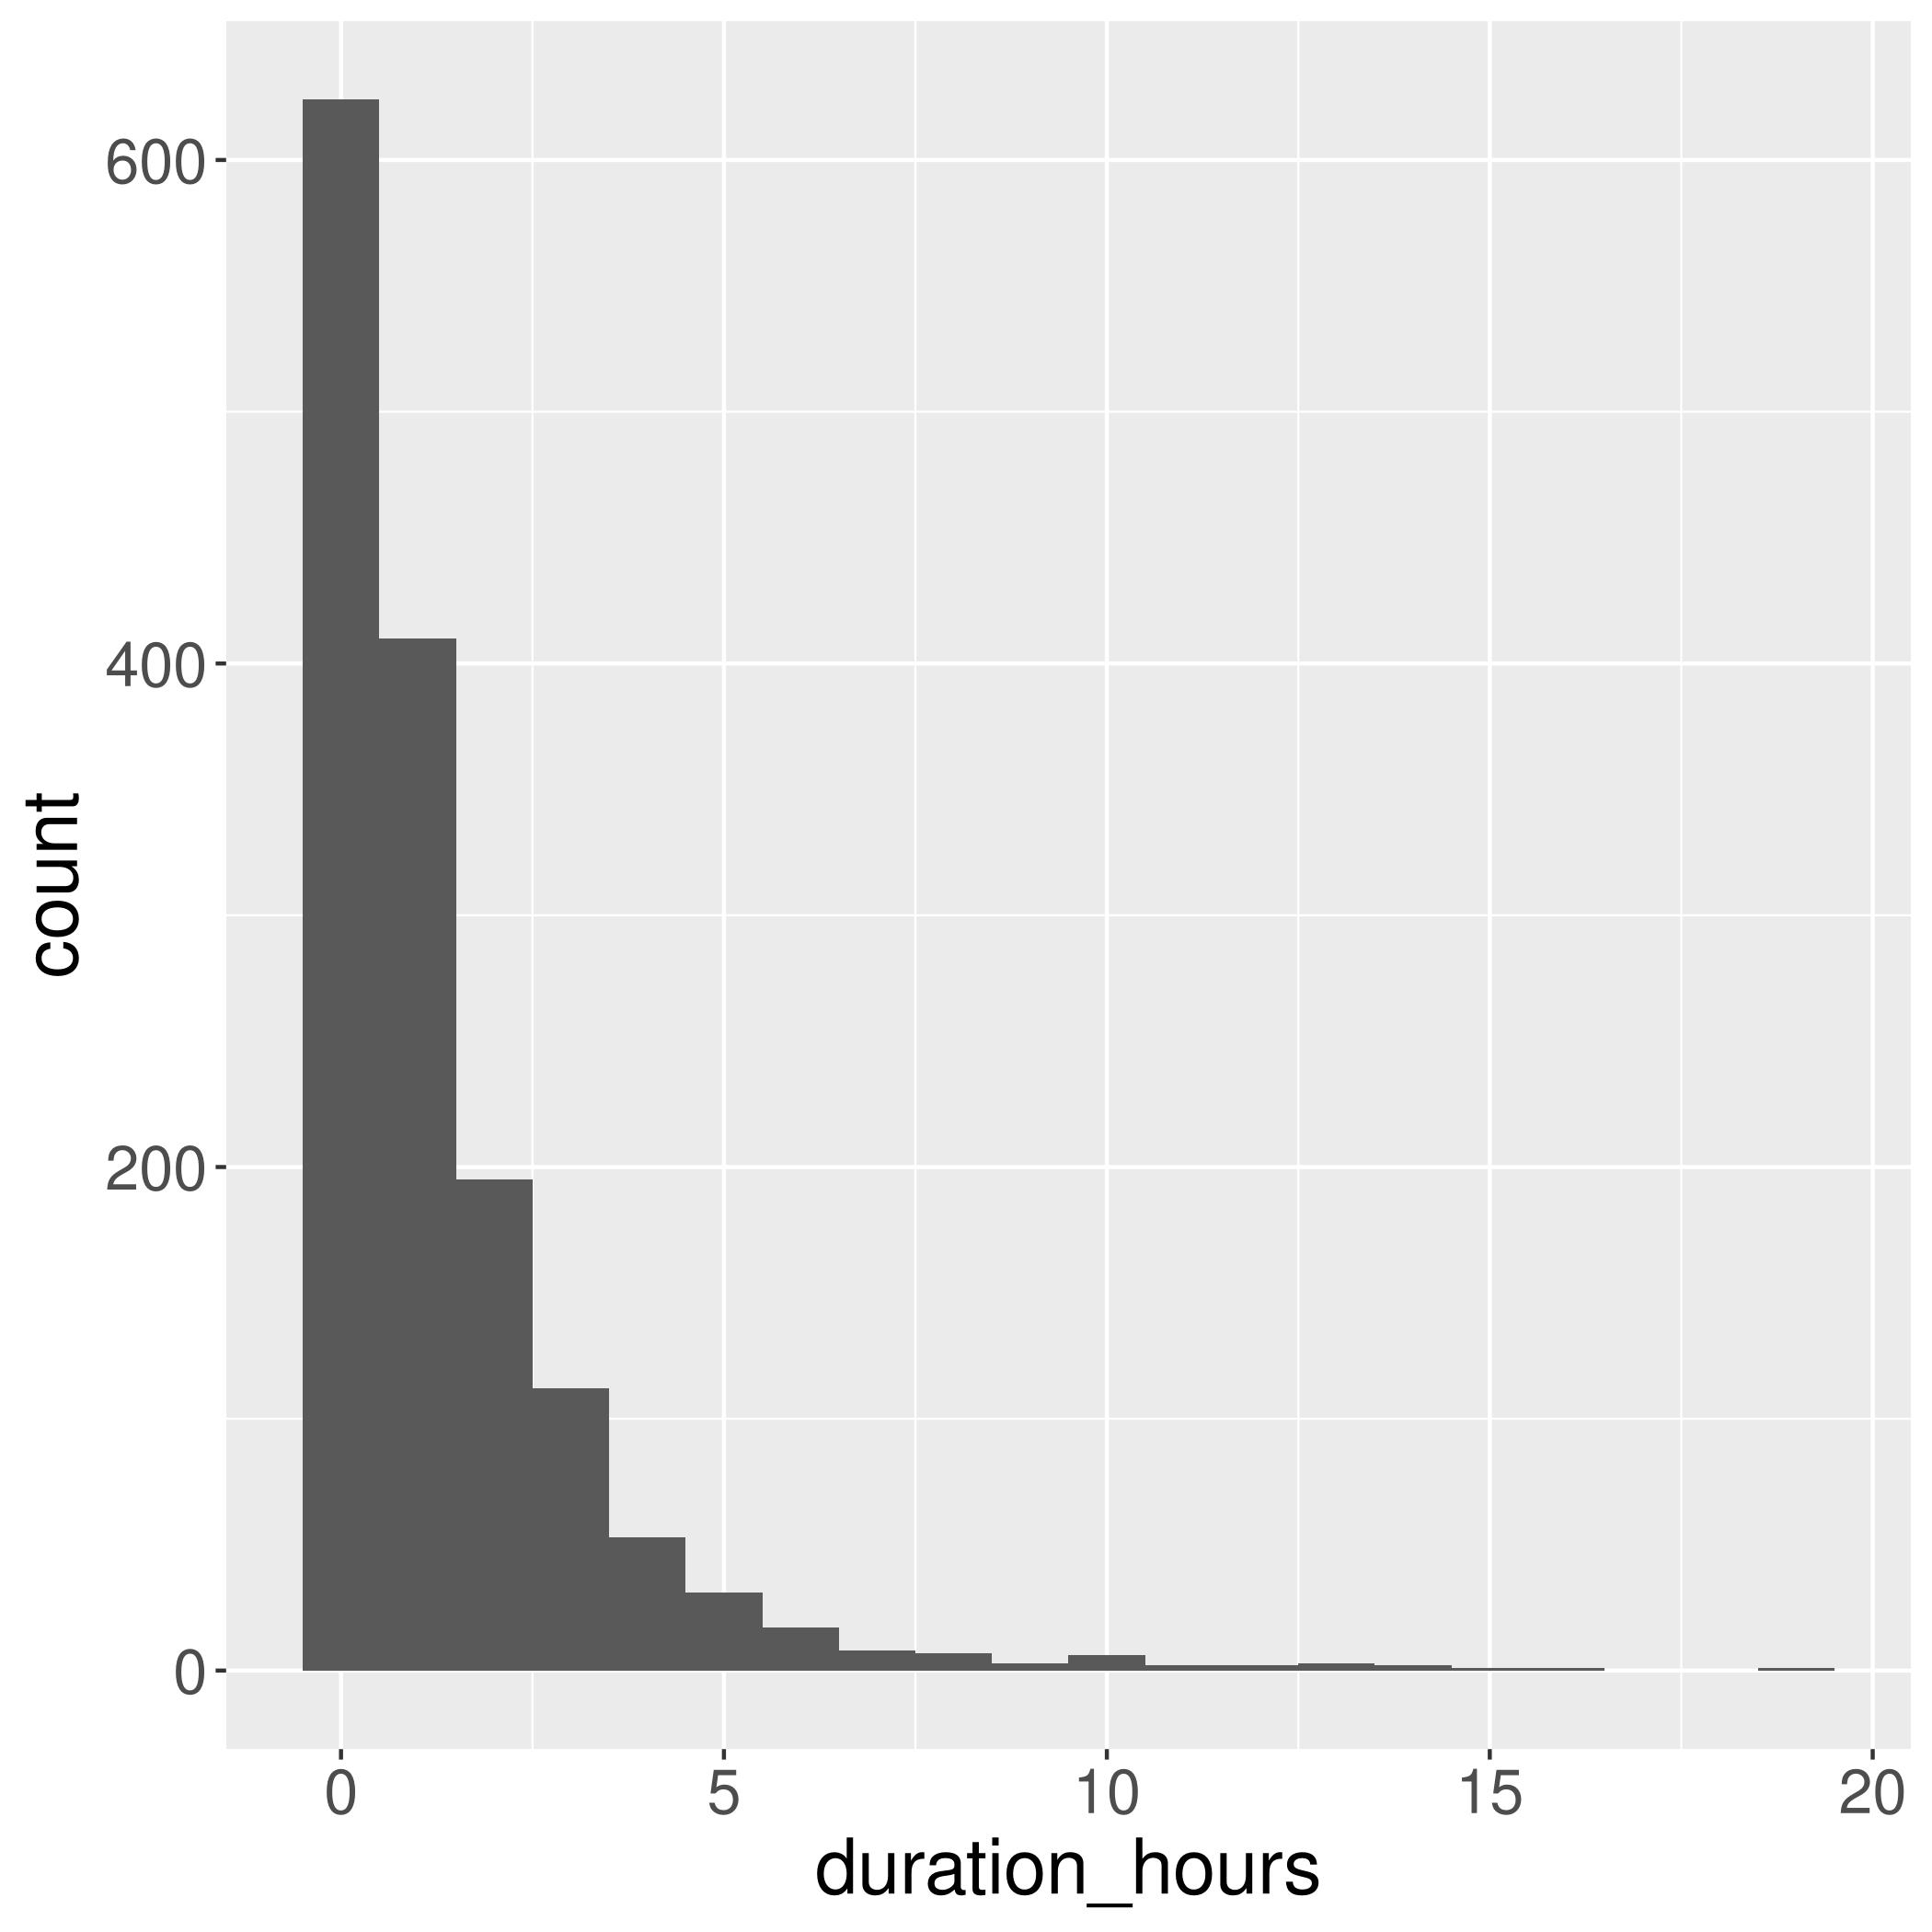
\includegraphics[width=.9\linewidth]{known_causes.jpg}
\end{center}
\end{itemize}
\subsection{Summarizing data}
\label{sec:orgda4338a}
\begin{verbatim}
  avg_delay_causes <- group_by(known_causes,cause_group) %>%
  summarize(avg=mean(duration_hours))

  ggplot(avg_delay_causes,aes(cause_group,avg)) +
  geom_bar(stat="identity")
\end{verbatim}

\begin{center}
  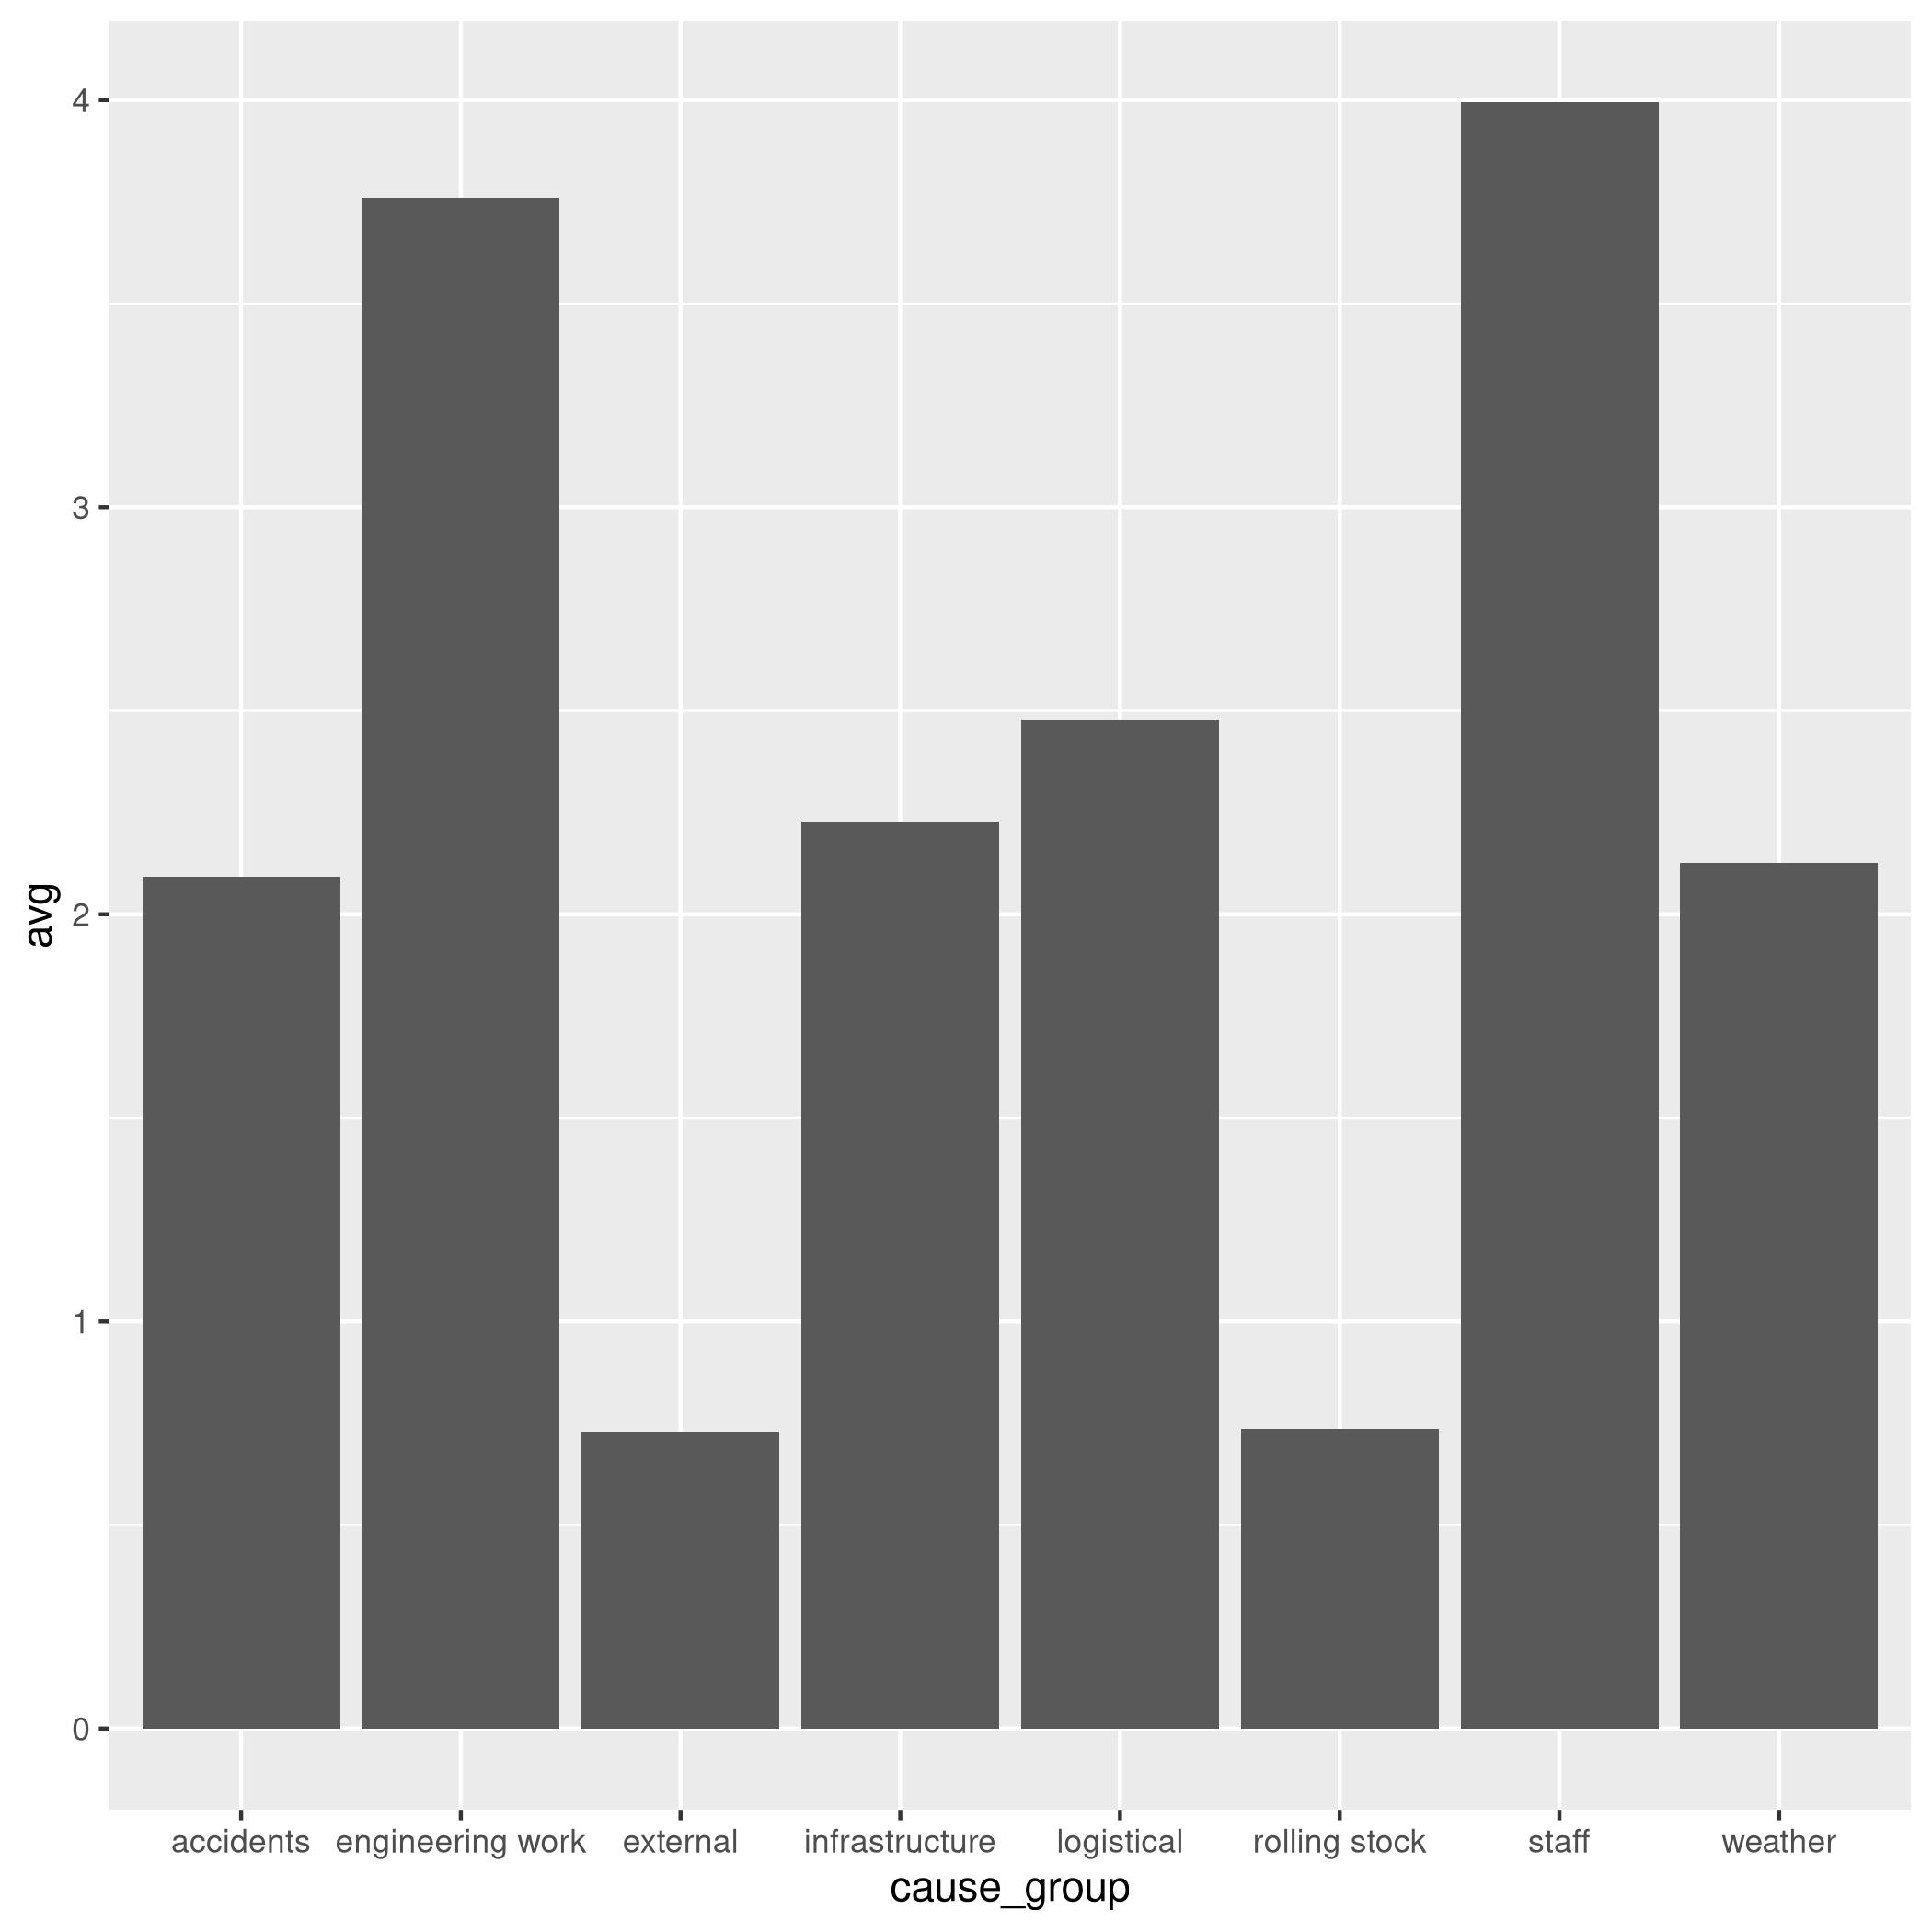
\includegraphics[width=.9\linewidth]{avg_delay_causes.jpg}
\end{center}

From this graph we can notice that the longer delays are usually due to "staff" cause, on the other hand
shorter delays are usually due to external or rolling stock causes.

\subsection{Spreading and gathering data}
\label{sec:org14dfec6}

In theory, the code below should gather the 1999 and 2000 columns into 2 new columns:
year and cases. In the column year the key of these columns will be insert (e.g. 1999 or 2000),
in the other column, cases,the value of associated with the key will be insert (e.g. 745 , 2666\ldots{}).
The firsts arguments to gather are similar to the select arguments.
The key argument is the name of the variable which values form the column key
The value argument is the associated value for that column

\begin{verbatim}
  table4a %>%
  gather(1999,2000,key = "year", value = "cases")
\end{verbatim}
It fails simply because there are missing backticks arround the numbers (they are non-syntactic names).
In the tibble they are store as character instead of numebers and therefore this line will always fails.
\begin{verbatim}

  people <- tribble(
  ~name,~key,~value,
  "Phillip Woods", "age", 45,
  "Phillip Woods","height",186,
  "Phillip Woods","age", 50,
  "Jessica Cordero","age",37,
  "Jessica Cordero","height",156)
  people %>%
  spread(key,value)
\end{verbatim}

the operation spread fails on the people tibble because there is not a unique combination
of keys which identify uniquely each row
\subsection{Separating \& uniting}
\label{sec:org016a55b}

"extra: If ‘sep’ is a character vector, this controls what happens
when there are too many pieces. There are three valid
options:

• "warn" (the default): emit a warning and drop extra
values.

• "drop": drop any extra values without a warning.

• "merge": only splits at most ‘length(into)’
times " (from the R help function)

"fill: If ‘sep’ is a character vector, this controls what happens
when there are not enough pieces. There are three valid
options:

• "warn" (the default): emit a warning and fill from the
right

• "right": fill with missing values on the right

• "left": fill with missing values on the left " (from the
R help function)

\begin{verbatim}
  tibble(x =c("a,b,c", "d,e,f,g", "h,i,j")) %>%
  separate(x,c("one", "two", "three"),extra="merge")
  # Result :
  # A tibble: 3 x 3
  #  one   two   three
  #  <chr> <chr> <chr>
  # 1 a     b     c
  # 2 d     e     f,g
  # 3 h     i     j

  tibble(x =c("a,b,c", "d,e", "f,g,i")) %>%
  separate(x,c("one", "two", "three"),fill="left")

  # Result:
  # A tibble: 3 x 3
  #  one   two   three
  #  <chr> <chr> <chr>
  # 1 a     b     c
  # 2 NA    d     e
  # 3 f     g     i
\end{verbatim}
\end{document}
